\chapter{Laravel Routing}

Routing เป็นการกำหนดวิธีการประมวลผลเมื่อมี Request (URL) เข้ามายัง Server แล้วส่ง Response กลับไป 
ซึ่งกำหนดการ Route ในไฟล์ \mintinline{bash}{routes/web.php} โดยต้องคำนึงถึงเรื่องต่าง ๆ ดังนี้

Request ที่เข้ามา เป็น HTTP Method ใด ซึ่งจะกำหนดชื่อฟังก์ชันของ Route ได้แก่
\bigskip
\begin{syntax}{php}{Routing Request Functions}{syntax:ch3:00}
    Route::get($uri, $callback);
    Route::post($uri, $callback);
    Route::put($uri, $callback);
    Route::patch($uri, $callback);
    Route::delete($uri, $callback);
    Route::options($uri, $callback);    
\end{syntax}
\medskip

Request ที่เข้ามา มาจาก URL path อะไร ซึ่งจะกำหนดเป็น parameter ที่ 1 
(\mintinline{php}{$uri}) หากเป็นคำที่ประกอบด้วยหลายคำ ให้ใช้ - เป็นตัวคั่น 
เช่น \mintinline{php}{/pages}, \mintinline{php}{/about-us}

จะ Response กลับด้วยวิธีใด ซึ่งจะกำหนดเป็น parameter ที่ 2 (\mintinline{php}{$callback})
\newpage

\section{ตัวอย่างการกำหนด routing}

ตัวอย่างการ response ด้วย Closure ที่ return String เมื่อมีการ request /hello
\begin{code}{php}{routes/web.php}{}
    <?php
    use Illuminate\Support\Facades\Route;

    Route::get('/hello', function () {
        return "Hello Laravel";
    });
\end{code}

\begin{figure}[h!]
    \centering
    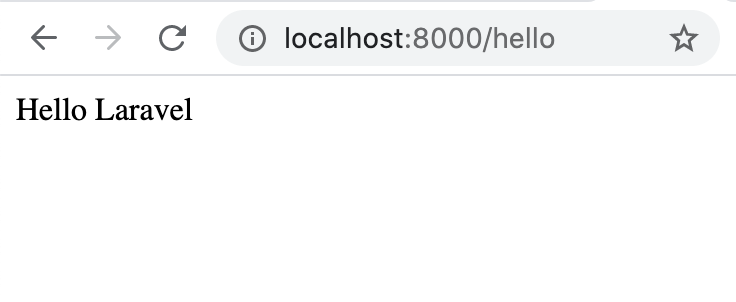
\includegraphics[width=0.6\textwidth]{images/ch2/02.png}
    \caption{หน้าเว็บที่เรียกไปยัง route /hello}
\end{figure}

ตัวอย่างการ response ด้วย Closure ที่ return Associative Array ซึ่งจะเปลี่ยนเป็น JSON
เมื่อมีการ request /hello/array
\begin{code}{php}{routes/web.php}{}
    <?php
    // ... 

    Route::get('/hello/array', function () {
        return [
            'message' => 'Hello Laravel', 
            'status' => 'success'
        ];
    });
\end{code}

\begin{figure}[h!]
    \centering
    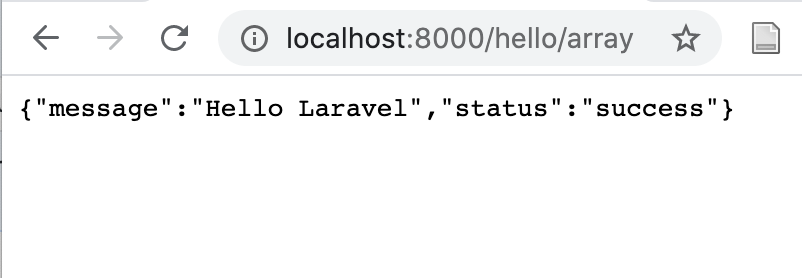
\includegraphics[width=0.6\textwidth]{images/ch2/03.png}
    \caption{หน้าเว็บที่เรียกไปยัง route /hello/array}
\end{figure}

ตัวอย่างการ response ด้วย Closure ที่ return view() โดยจะต้องส่งชื่อไฟล์ .blade.php 
ที่อยู่ใน directory \mintinline{bash}{resources/views} เป็น parameter ของฟังก์ชัน \mintinline{php}{view()}

\begin{code}{php}{routes/web.php}{}
    <?php
    // ...
    Route::get('/', function () {
        return view('welcome'); # resources/views/welcome.blade.php
    });
\end{code}

\begin{figure}[h!]
    \centering
    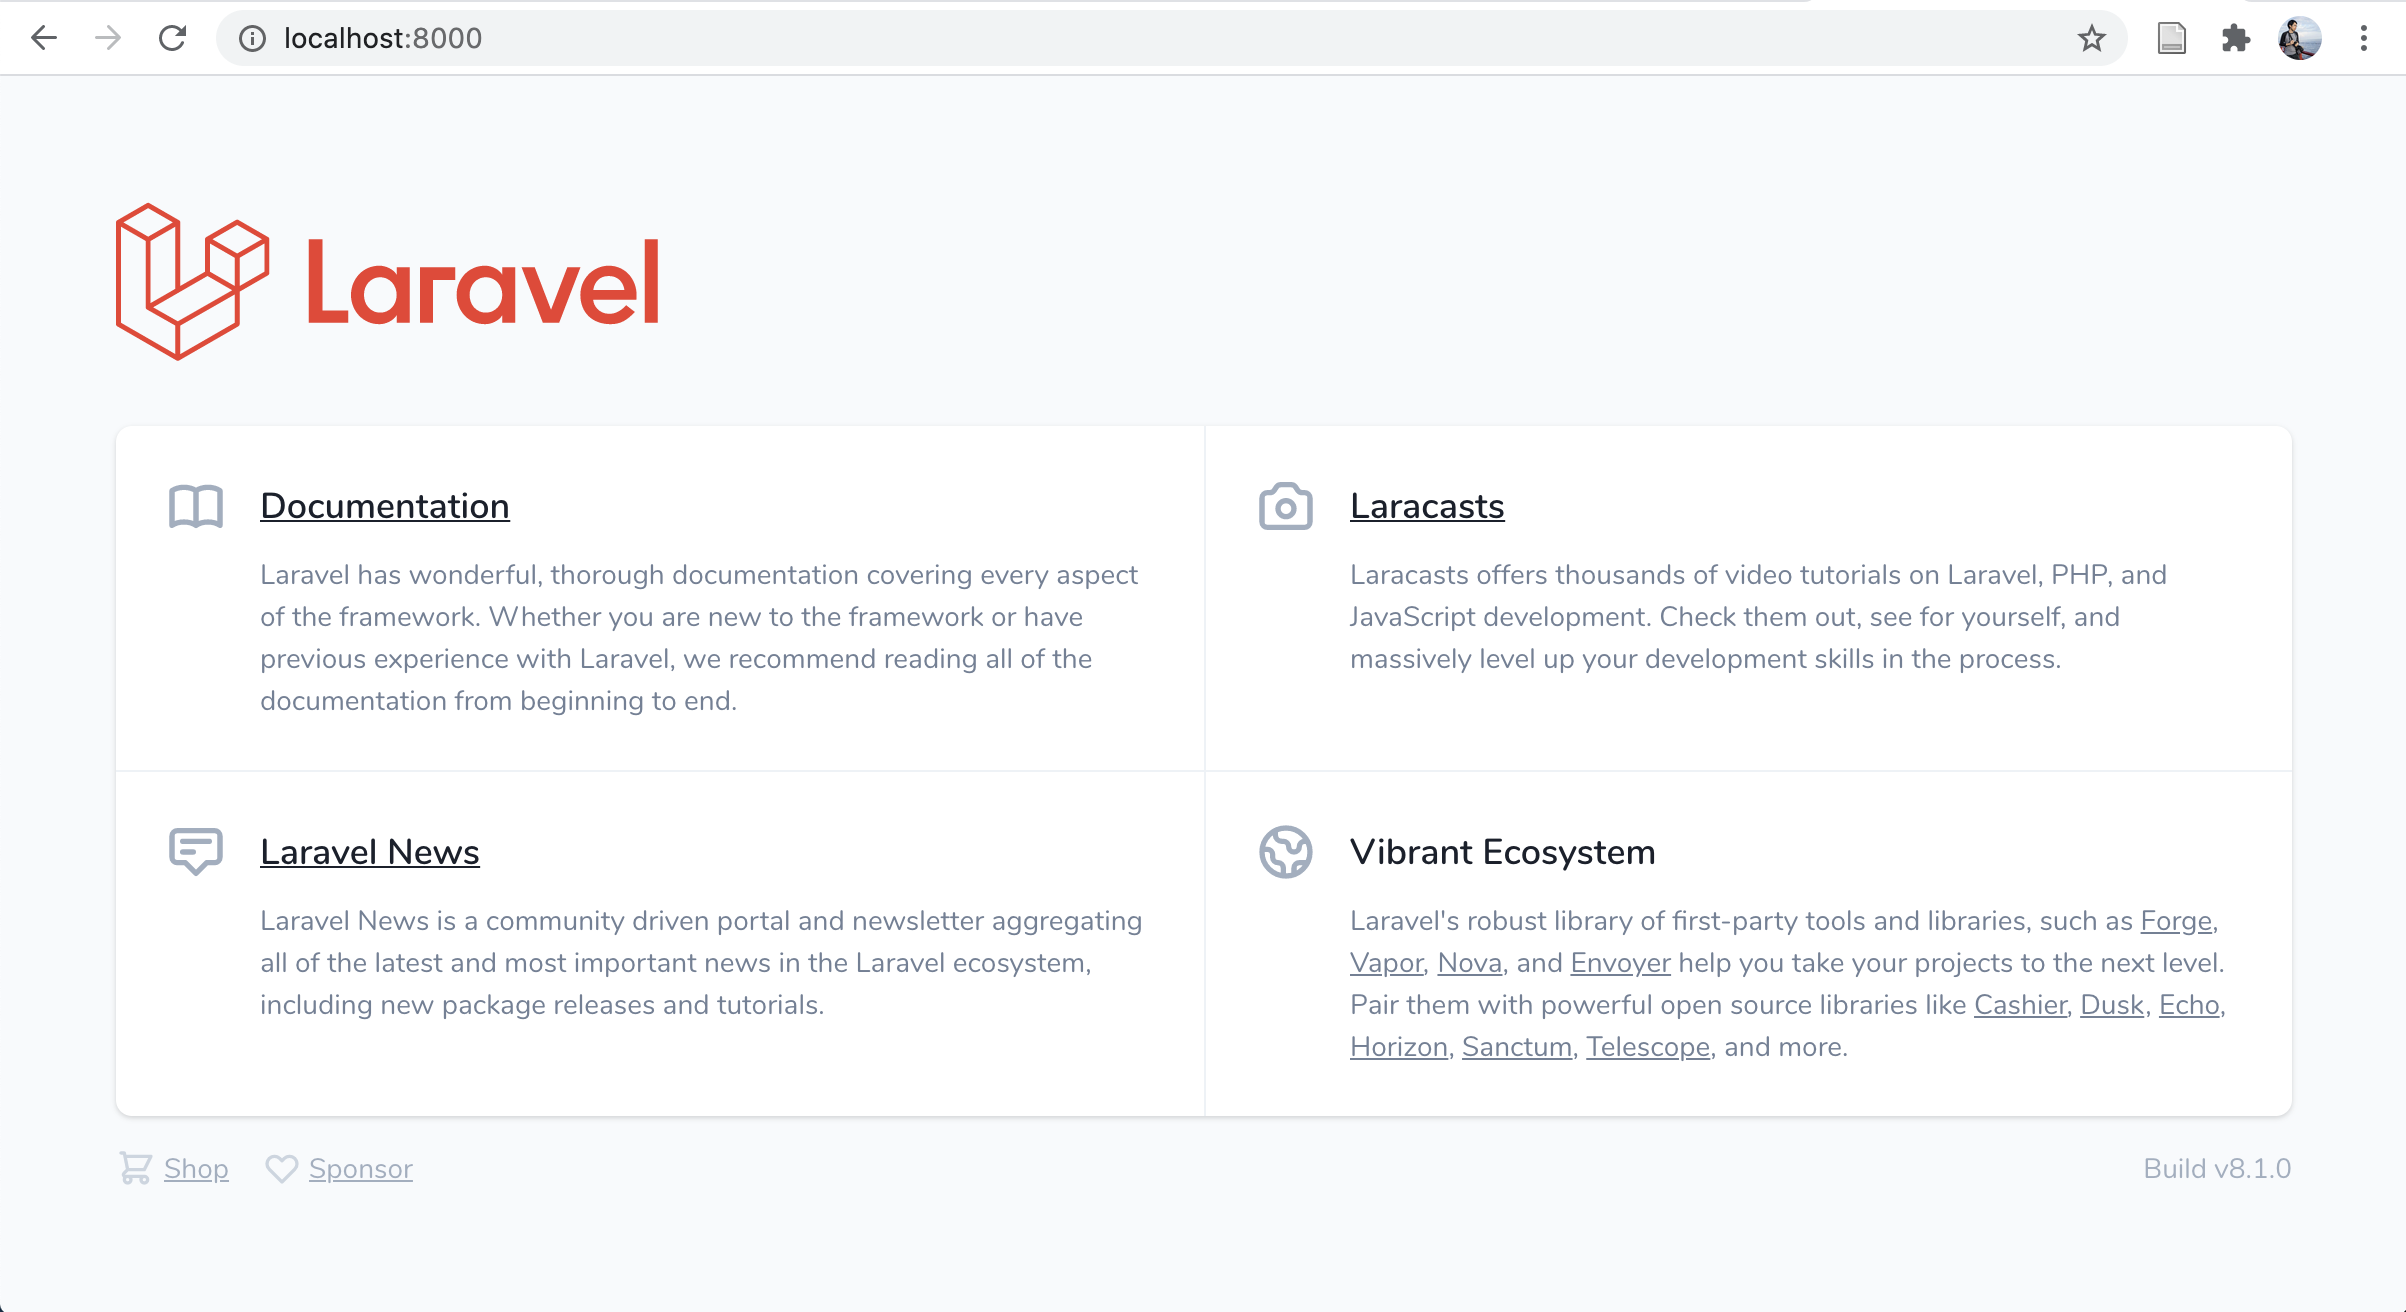
\includegraphics[width=1\textwidth]{images/ch2/01.png}
    \caption{หน้าเว็บที่เรียกไปยัง route /}
\end{figure}

\section{Route: Required Parameters}
การกำหนด parameter ของ request URL path ทำได้โดยระบุชื่อ parameter ในเครื่องหมาย \mintinline{php}{{}} ที่ Route path 
และระบุ parameter name ใน closure ด้วย เช่น

\begin{code}{php}{routes/web.php}{}
    <?php
    // ...
    Route::get('/pages/{id}', function ($id) {
        return [
            'Page ID' => $id
        ];
    });
\end{code}

ชื่อที่ระบุใน \mintinline{php}{{}} จะต้องเป็นตัวอักษรประเภท alphabetic และไม่ใช้ - ให้เลี่ยงไปใช้ underscore (\mintinline{php}{_})

\begin{figure}[h!]
    \centering
    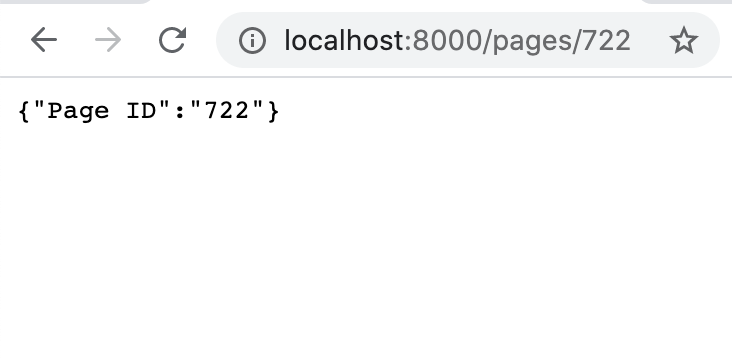
\includegraphics[width=0.6\textwidth]{images/ch3/04.png}
    \caption{หน้าเว็บที่เรียกไปยัง route /pages/722}
\end{figure}

\begin{figure}[h!]
    \centering
    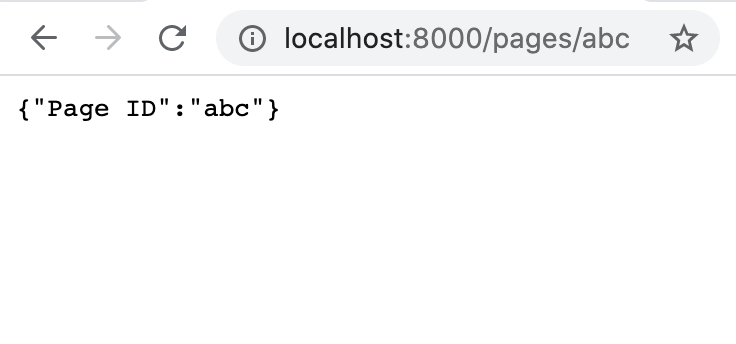
\includegraphics[width=0.6\textwidth]{images/ch3/05.png}
    \caption{หน้าเว็บที่เรียกไปยัง route /pages/abc}
\end{figure}

เมื่อกำหนด required parameter แล้ว แต่ request URL path ไม่ระบุ parameter นั้น
จะ response ว่าไม่พบหน้าที่ต้องการ

\begin{figure}[h!]
    \centering
    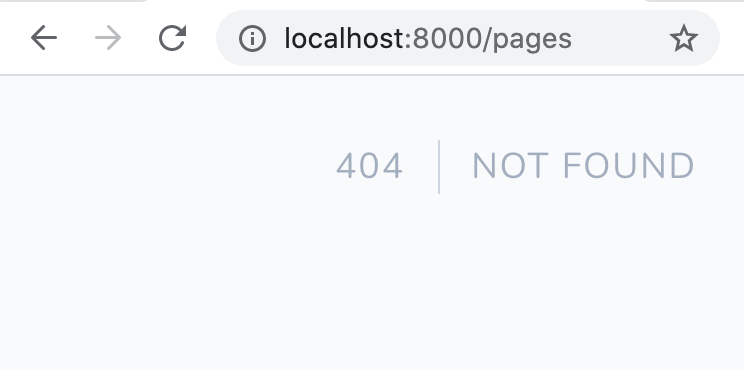
\includegraphics[width=0.6\textwidth]{images/ch3/06.png}
    \caption{หน้าเว็บที่เรียกไปยัง route /pages แต่ไม่ระบุส่วน required id}
\end{figure}

\section{Route: Optional Parameters}

กรณีที่ parameter ของ request URL path เป็น optional ให้ใส่ \mintinline{php}{?} หลังชื่อที่ระบุใน \mintinline{php}{{}} 
ของ URL path และกำหนด default value ของ parameter ใน closure เช่น

\begin{code}{php}{routes/web.php}{}
    <?php
    // ...
    Route::get('/pages/{id?}', function ($id = null) {
        return [
            'Page ID' => $id
        ];
    });
\end{code}

\newpage

\begin{figure}[h!]
    \centering
    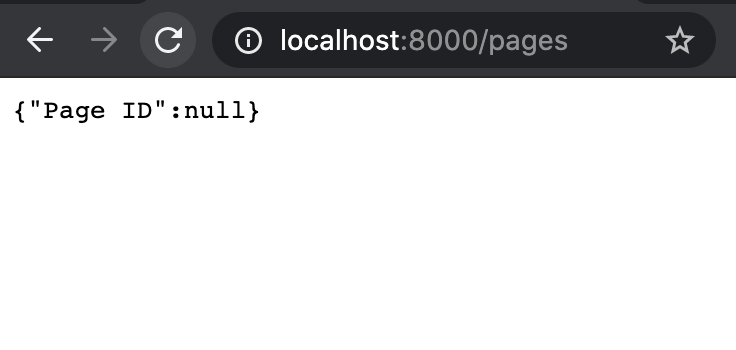
\includegraphics[width=0.6\textwidth]{images/ch3/07.png}
    \caption{หน้าเว็บที่เรียกไปยัง route /pages แต่ไม่ระบุส่วน optional id}
\end{figure}

Routing รูปแบบอื่น ศึกษาได้ที่ https://laravel.com/docs/8.x/routing

\subsection{การตรวจสอบ Route ทั้งหมดของระบบ}

คำสั่งสำหรับตรวจสอบ Routing ทั้งหมด ของ Laravel Project

\begin{cli}{}
    php artisan route:list
\end{cli}

\begin{out}{}
+--------+----------+-------------+------+---------+------------+
| Domain | Method   | URI         | Name | Action  | Middleware |
+--------+----------+-------------+------+---------+------------+
|        | GET|HEAD | /           |      | Closure | web        |
|        | GET|HEAD | api/user    |      | Closure | api        |
|        |          |             |      |         | auth:api   |
|        | GET|HEAD | hello       |      | Closure | web        |
|        | GET|HEAD | hello/array |      | Closure | web        |
|        | GET|HEAD | pages/{id?} |      | Closure | web        |
+--------+----------+-------------+------+---------+------------+
\end{out}